\chapter{Design and Implementation}

\section{Technologies Used}

Framework:

\begin{itemize}
\item Swift - Swift is the most modern language used for producing native iOS apps.  It is more readable and flexible than Obj-C, making it a better choice for this project. It is also backwards compatible with Obj-C and C++ libraries so it does not limit the usage of open source material in the system. It is used for the framework as well as the trilateration calculations.
\end{itemize}

Admin Webservice:

\begin{itemize}
\item HTML/CSS - Will be used for formatting and styling of admin webpage.
\item Javascript and JQuery - Javascript was used to add responsiveness and to provide underlying front end logic. JQuery was used to simplify DOM manipulation of admin webpage and AJAX calls.
\item PHP - Used on the back end of the admin web service to sanitize inputs and interface with the database.
\item MySQL - Used for the datastore of the admin web service.
\item Google Maps API - Used for abstract mapping of floor plan to real life latitude and longitude.
\end{itemize}

Network:
\begin{itemize}
\item iBeacon - the iBeacon protocol will be used in all broadcasting beacons
\end{itemize}

\begin{figure}
\section{Architectural Diagram}
The following architectural diagram shows that the framework conceptually is built on top of the iOS CoreLocation service.  The admin web app will only have to be reachable by the framework during the initial phase of the system installation or when major changes are made to the system.
\newline
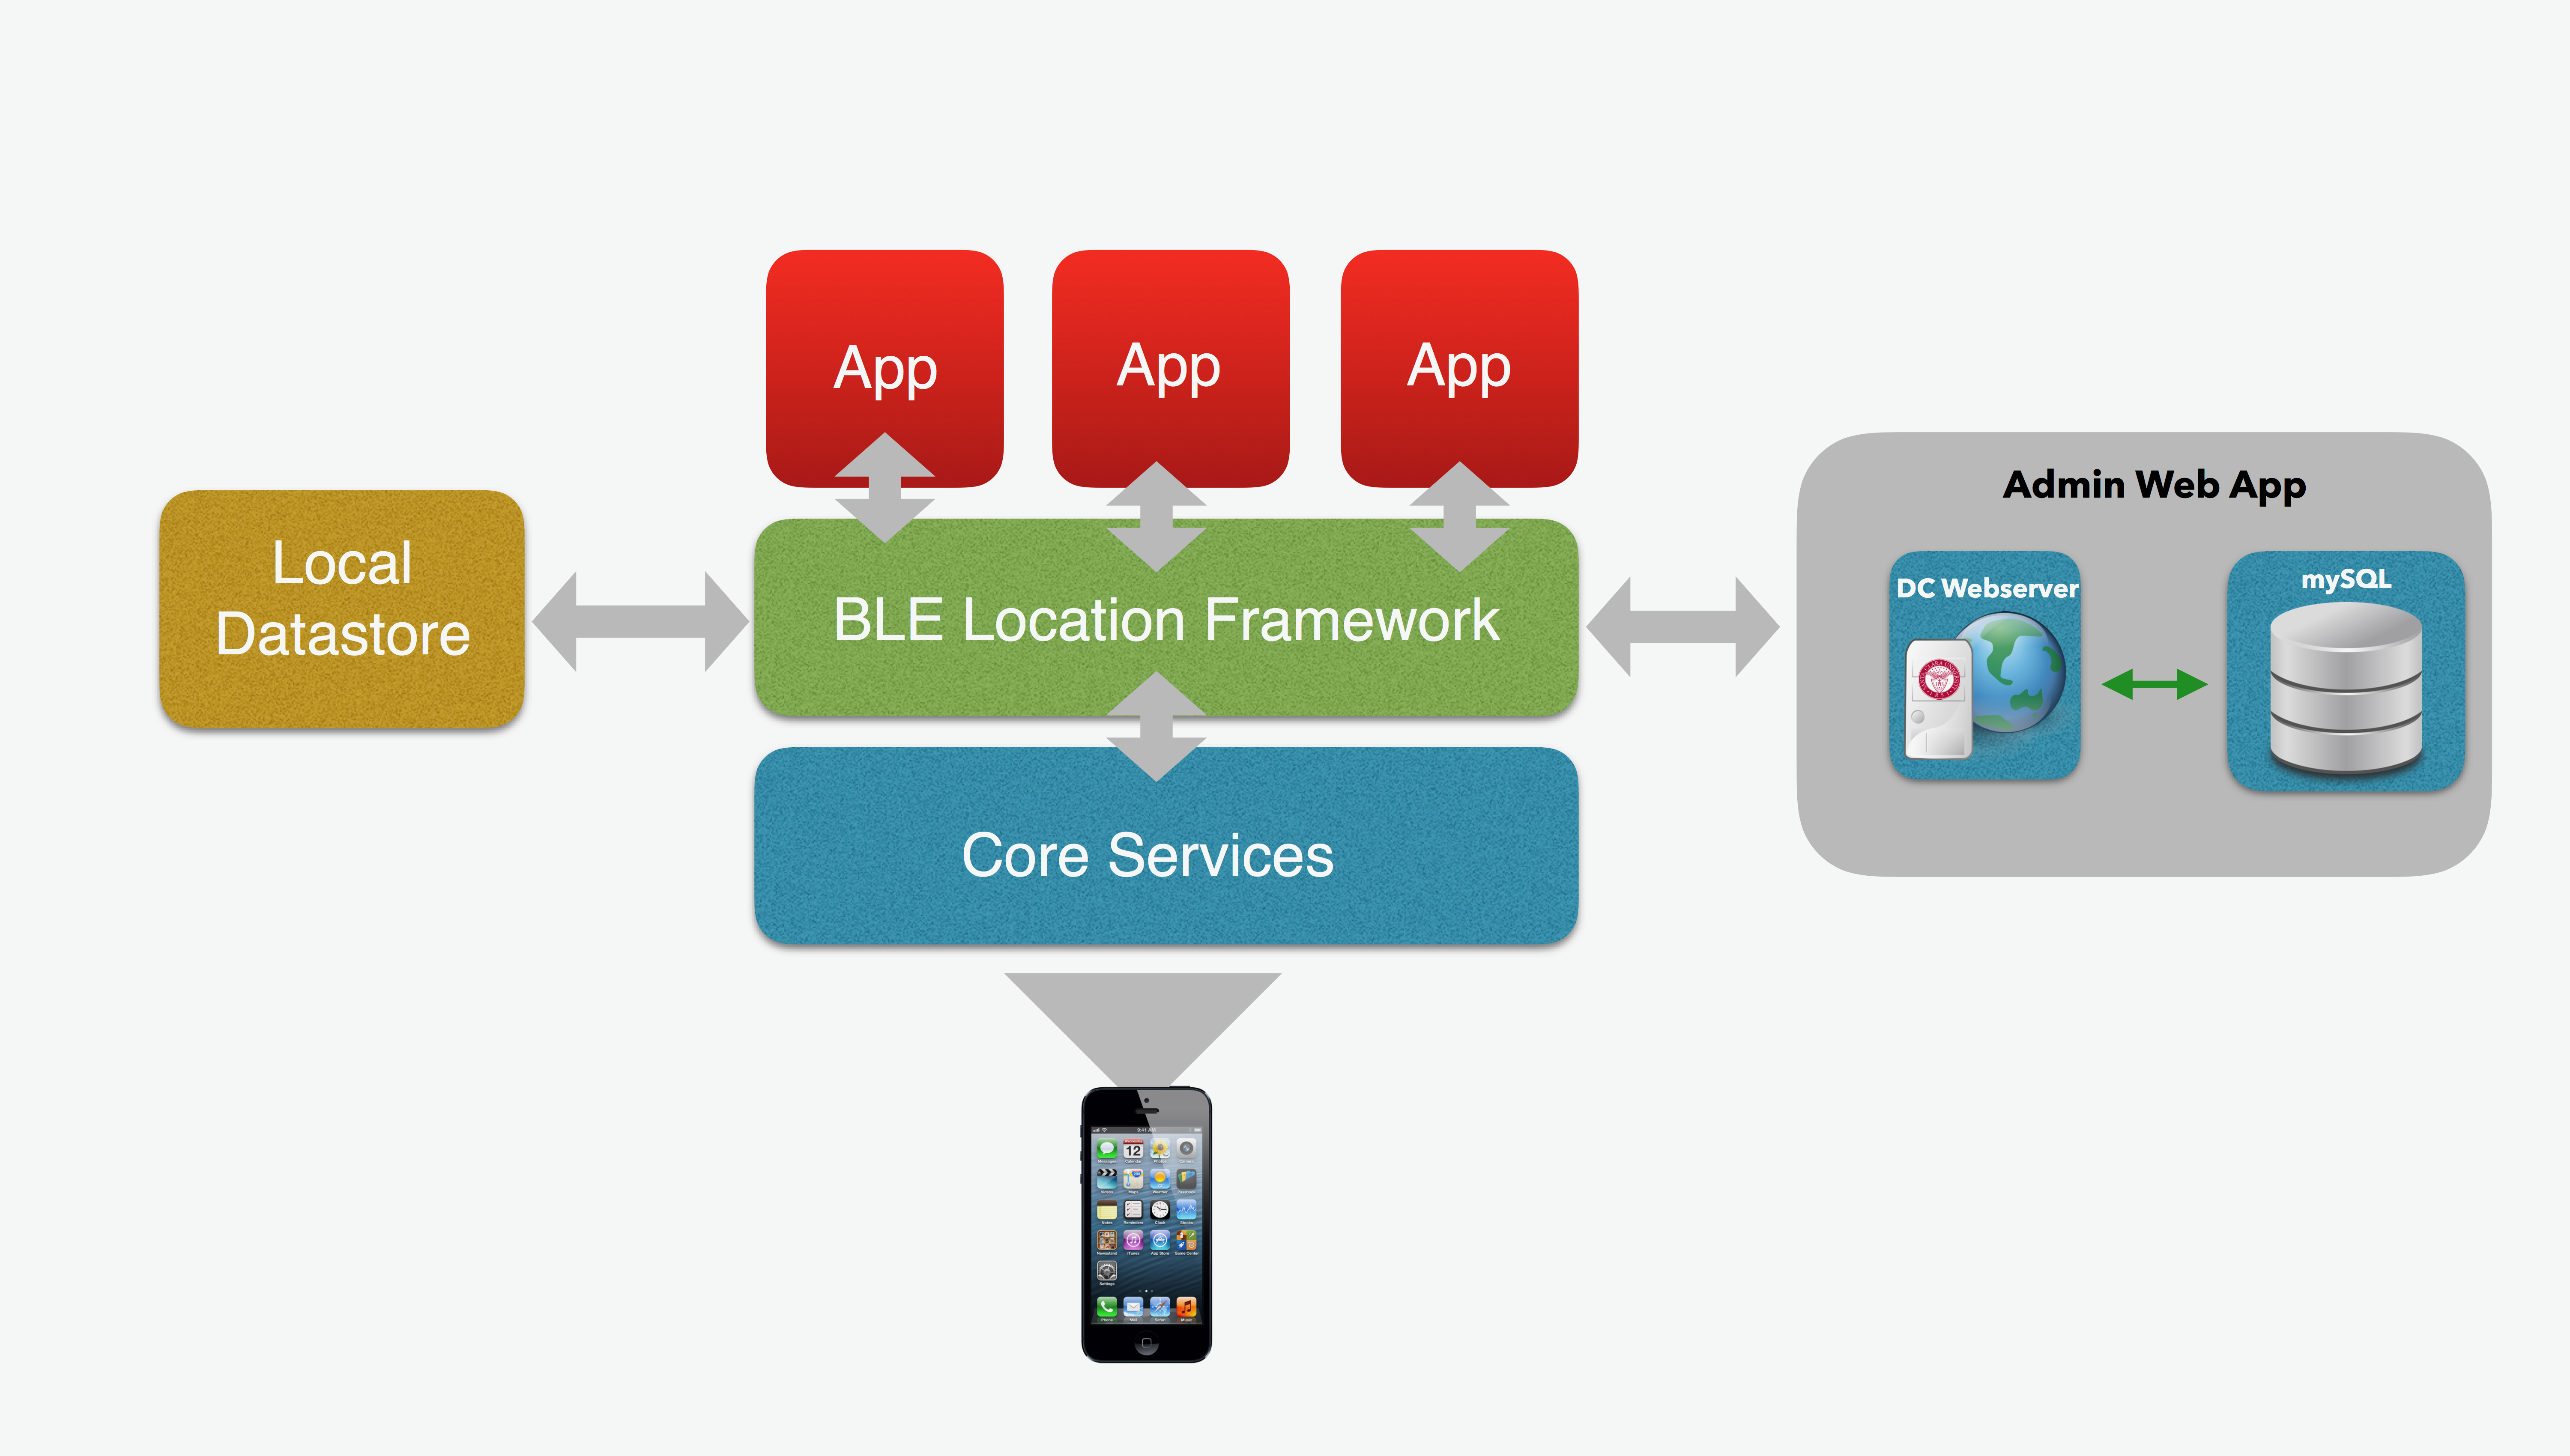
\includegraphics[width=1\textwidth]{images/arch.png}
\caption{Architectural Diagram}
\end{figure}
